\documentclass{standalone}
\usepackage{tikz}

\begin{document}
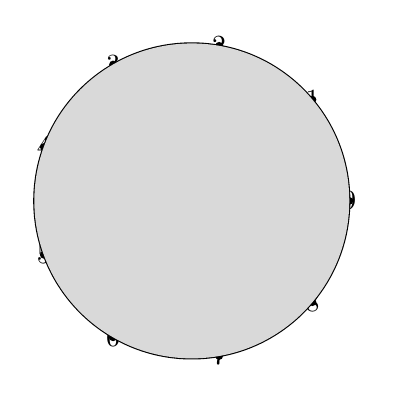
\begin{tikzpicture}[scale=2]
    % Draw the circle
    \draw[thick] (0,0) circle (1);

    % Place numbers around the circle
    \foreach \i in {1,...,9} {
        \node[circle, fill=black, inner sep=1pt] at ({cos(\i*40)}, {sin(\i*40)}) {};
        \node at ({cos(\i*40)}, {sin(\i*40)}) {\i};
    }

    % Draw the chords
    \draw[dashed, thick] (1,0) -- (-0.5,-0.866);
    \draw[dashed, thick] (0.5,-0.866) -- (0,0);
    \draw[dashed, thick] (0,0) -- (0.5,0.866);
    \draw[dashed, thick] (0.5,0.866) -- (1,0);
    \draw[dashed, thick] (-0.5,0.866) -- (0,0);
    \draw[dashed, thick] (0,0) -- (-0.5,-0.866);
    \draw[dashed, thick] (0.5,0.866) -- (-0.5,-0.866);
    \draw[dashed, thick] (0.5,-0.866) -- (0.5,0.866);
    \draw[dashed, thick] (-0.5,0.866) -- (-0.5,-0.866);

    % Fill the circle with alternating colors
    \fill[gray!30] (0,0) circle (1);
\end{tikzpicture}
\end{document}